\subsection{PROPERTIES OF THE GAMMA FUNCTION}

PROPOSITION 2. For every x \textgreater{} 0 one has

\[
\Gamma (x) = \lim _ {n \rightarrow \infty} \frac {n ^ {x} n !}{x (x + 1) \dots (x + n)}\tag{8}
\]

(Gauss' formula), and

\[
\Gamma (x) = e ^ {- \gamma x} \frac {1}{x} \prod_ {n = 1} ^ {\infty} \frac {e ^ {x / n}}{1 + \frac {x}{n}}\tag{9}
\]

where \(\gamma\) denotes Euler's constant, and the infinite product on the right hand side of (9) is absolutely and uniformly convergent on every compact interval of \(\mathbf{R}\) not containing any integer \(< 0\) (Weierstrass' formula).

The function \(\Gamma(x)\) is indefinitely differentiable on \(]0, +\infty[\) and one has

\[
{\frac {\Gamma^ {\prime} (x)}{\Gamma (x)}} = - \gamma - {\frac {1}{x}} + \sum_ {n = 1} ^ {\infty} \left({\frac {1}{n}} - {\frac {1}{x + n}}\right)\tag{10}
\]

and

\[
\mathrm{D} ^ {k} (\log \Gamma (x)) = \sum_ {n = 0} ^ {\infty} \frac {(- 1) ^ {k} (k - 1) !}{(x + n) ^ {k}} \quad \text { for } \quad k \geqslant 2,\tag{11}
\]

the series on the right-hand sides of (10) and (11) being absolutely and uniformly convergent on every compact interval not containing any integer \(\leqslant 0\) .

Indeed, the proof of prop. 1 of VII, p.~306, shows that

\[
\Gamma (x) = \lim _ {n \rightarrow \infty} \frac {n ^ {x} (n - 1) !}{x (x + 1) \dots (x + n - 1)}
\]

whence Gauss' formula, since \(\frac{n}{x + n}\) tends to 1 as \(n\) tends to \(+\infty\) . One can also write

\[
\log \frac {n}{n - 1} = \frac {1}{n - 1} + \left(\log \frac {n}{n - 1} - \frac {1}{n - 1}\right),
\]

so (in the notation of prop. 1)

\[
\exp (u _ {n} (x)) = e ^ {x \left(\log \frac {n}{n - 1} - \frac {1}{n - 1}\right)} \frac {e ^ {x / n - 1}}{1 + \frac {x}{n - 1}}
\]

and the series with general term \(\log \frac{n}{n - 1} -\frac{1}{n - 1}\) is absolutely convergent and has sum \(-\gamma\) , where \(\gamma\) denotes Euler's constant (V,p.242), whence we obtain Weierstrass' formula.

For \(|x| \leqslant a\) one has \(\left|1/(x+n)^{k}\right| \leqslant 1/(n-a)^{k}\) once n \textgreater{} a, so the series on the right-hand side in formula (11) is absolutely and uniformly convergent on every compact interval of R not containing any integer \(\leqslant 0\) , for any integer \(k \geqslant 2\) ; the same argument applies to the right-hand side of (10), since \(\left|\frac{1}{n}-\frac{1}{x+n}\right| \leqslant \frac{a}{n(n-a)}\) for \(|x| \leqslant a\) and n \textgreater{} a. Since these series are obtained by differentiating the series

\[
\log \Gamma (x) = - \gamma x - \log x + \sum_ {n = 1} ^ {\infty} \left(\frac {x}{n} - \log \left(1 + \frac {x}{n}\right)\right)
\]

term-by-term, and this converges for every \(x > 0\) , the series with general term \(\frac{x}{n} - \log \left(1 + \frac{x}{n}\right)\) is absolutely and uniformly convergent on every compact interval contained in \([0, +\infty[\) , and one has the relations (10) and (11) of VII, p.~308, for every x \textgreater{} 0 (II, p.~52, th. 1). Moreover, for every \(x \in R\) , the expression \(\frac{x}{n} - \log\left(1 + \frac{x}{n}\right)\) is defined once n is large enough, so th. 1 of II, p.~52, again shows that the infinite product in the right-hand side of (9) (VII, p.~307) is absolutely and uniformly convergent on every compact interval containing no integer \(\leqslant 0\) .

The function \(\Gamma(x)\) , defined for x \textgreater{} 0, can be extended to the whole set of points x different from the integers \(\leqslant 0\) so as to satisfy equation (7) of VII, p.~307, on this set: it suffices, for \(-(n + 1) < x < -n\) , to put

\[
\Gamma (x) = \frac {1}{x (x + 1) \ldots (x + n)} \Gamma (x + n + 1).
\]

By prop. 2 of VII, p.~307, the formulae (8), (9), (10) and (11) of VII, p.~307 and 308, with \(\mathrm{D}^{k}(\log|\Gamma(x)|)\) replacing \(\mathrm{D}^{k}(\log\Gamma(x))\) in (11), remain valid on this set. Formula (9) (VII, p.~307) shows that \(\Gamma(x)\sim1/x\) as x tends to 0, whence, by (7) of VII, p.~307,

\[
\Gamma (x) \sim \frac {(- 1) ^ {n}}{n ! (x + n)}
\]

as \(x\) tends to \(-n\) ( \(n\) an integer \(\geqslant 0\) ). The function \(1 / \Gamma(x)\) can then be extended by continuity to all of \(\mathbf{R}\) , assigning it the value 0 at integers \(\leqslant 0\) ; then, for all \(x \in \mathbf{R}\)

\[
\frac {1}{\Gamma (x)} = \lim _ {n \rightarrow \infty} \frac {x (x + 1) \dots (x + n)}{n ^ {x} n !}\tag{12}
\]

and

\[
\frac {1}{\Gamma (x)} = e ^ {\gamma x} x \prod_ {n = 1} ^ {\infty} \left(1 + \frac {x}{n}\right) e ^ {- x / n}\tag{13}
\]

and one shows as in prop. 2 of VII, p.~307, that the infinite product on the right of (13) is absolutely and uniformly convergent on every compact interval of \(\mathbf{R}\) .

Since \(\Gamma(x) > 0\) for \(x > 0\) , equation (7) of VII, p.~307, shows that \(\Gamma(x) < 0\) for \(-(2n - 1) < x < -(2n - 2)\) and \(\Gamma(x) > 0\) for

\[
- 2 n <   x <   - (2 n - 1)
\]

\((n \text{ an integer } \geqslant 1); \text{ also } \Gamma(x) \text{ has right limit } +\infty \text{ at the points } -2n \text{ and } -\infty \text{ at the points } -(2n+1), \text{ and has left limit } -\infty \text{ at the points } -2n \text{ and } +\infty \text{ at the points } -(2n+1) \text{ (for all } n \in \mathbf{N}). \text{ Formula (11) of VII, p. 308, shows that, for } k=2, \text{ the right-hand side is always } \geqslant 0 \text{ when it is defined, so}\)

\[
\Gamma^ {\prime \prime} (x) \Gamma (x) - \left(\Gamma^ {\prime} (x)\right) ^ {2} \geqslant 0,
\]

\pandocbounded{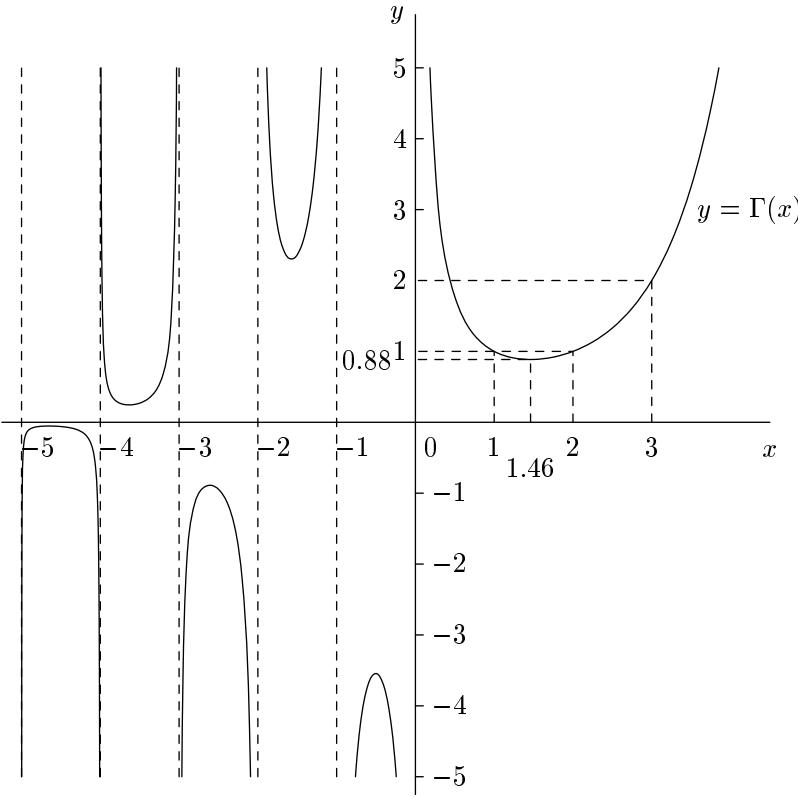
\includegraphics[keepaspectratio]{images/part002_cfbcc1f6.jpg}}\\
Fig. 1\\
and consequently \(\Gamma''(x)\) has the same sign as \(\Gamma(x)\) ; thus \(\Gamma\) is convex for x \textgreater{} 0 and for \(-(2n + 2) < x < -(2n + 1)\) , and concave for \(-(2n + 1) < x - 2n\) ( \(n \in N\) ); one deduces from this that, on the intervals where \(\Gamma\) is convex, \(\Gamma'(x)\) increases from \(-\infty\) to \(+\infty\) , and on the intervals where \(\Gamma\) is concave, \(\Gamma'(x)\) decreases from \(+\infty\) to \(-\infty\) . Whence the graph of \(\Gamma\) (fig.~1).
% semantic-fragments: legacy-input-seam
\relax{}
